\documentclass[twoside]{book}

% Packages required by doxygen
\usepackage{fixltx2e}
\usepackage{calc}
\usepackage{doxygen}
\usepackage[export]{adjustbox} % also loads graphicx
\usepackage{graphicx}
\usepackage[utf8]{inputenc}
\usepackage{makeidx}
\usepackage{multicol}
\usepackage{multirow}
\PassOptionsToPackage{warn}{textcomp}
\usepackage{textcomp}
\usepackage[nointegrals]{wasysym}
\usepackage[table]{xcolor}

% Font selection
\usepackage[T1]{fontenc}
\usepackage[scaled=.90]{helvet}
\usepackage{courier}
\usepackage{amssymb}
\usepackage{sectsty}
\renewcommand{\familydefault}{\sfdefault}
\allsectionsfont{%
  \fontseries{bc}\selectfont%
  \color{darkgray}%
}
\renewcommand{\DoxyLabelFont}{%
  \fontseries{bc}\selectfont%
  \color{darkgray}%
}
\newcommand{\+}{\discretionary{\mbox{\scriptsize$\hookleftarrow$}}{}{}}

% Page & text layout
\usepackage{geometry}
\geometry{%
  a4paper,%
  top=2.5cm,%
  bottom=2.5cm,%
  left=2.5cm,%
  right=2.5cm%
}
\tolerance=750
\hfuzz=15pt
\hbadness=750
\setlength{\emergencystretch}{15pt}
\setlength{\parindent}{0cm}
\setlength{\parskip}{3ex plus 2ex minus 2ex}
\makeatletter
\renewcommand{\paragraph}{%
  \@startsection{paragraph}{4}{0ex}{-1.0ex}{1.0ex}{%
    \normalfont\normalsize\bfseries\SS@parafont%
  }%
}
\renewcommand{\subparagraph}{%
  \@startsection{subparagraph}{5}{0ex}{-1.0ex}{1.0ex}{%
    \normalfont\normalsize\bfseries\SS@subparafont%
  }%
}
\makeatother

% Headers & footers
\usepackage{fancyhdr}
\pagestyle{fancyplain}
\fancyhead[LE]{\fancyplain{}{\bfseries\thepage}}
\fancyhead[CE]{\fancyplain{}{}}
\fancyhead[RE]{\fancyplain{}{\bfseries\leftmark}}
\fancyhead[LO]{\fancyplain{}{\bfseries\rightmark}}
\fancyhead[CO]{\fancyplain{}{}}
\fancyhead[RO]{\fancyplain{}{\bfseries\thepage}}
\fancyfoot[LE]{\fancyplain{}{}}
\fancyfoot[CE]{\fancyplain{}{}}
\fancyfoot[RE]{\fancyplain{}{\bfseries\scriptsize Generated by Doxygen }}
\fancyfoot[LO]{\fancyplain{}{\bfseries\scriptsize Generated by Doxygen }}
\fancyfoot[CO]{\fancyplain{}{}}
\fancyfoot[RO]{\fancyplain{}{}}
\renewcommand{\footrulewidth}{0.4pt}
\renewcommand{\chaptermark}[1]{%
  \markboth{#1}{}%
}
\renewcommand{\sectionmark}[1]{%
  \markright{\thesection\ #1}%
}

% Indices & bibliography
\usepackage{natbib}
\usepackage[titles]{tocloft}
\setcounter{tocdepth}{3}
\setcounter{secnumdepth}{5}
\makeindex

% Custom commands
\newcommand{\clearemptydoublepage}{%
  \newpage{\pagestyle{empty}\cleardoublepage}%
}

\usepackage{caption}
\captionsetup{labelsep=space,justification=centering,font={bf},singlelinecheck=off,skip=4pt,position=top}

%===== C O N T E N T S =====

\begin{document}

% Titlepage & ToC
\pagenumbering{alph}
\begin{titlepage}
\vspace*{7cm}
\begin{center}%
{\Large H\+RD \\[1ex]\large 1.\+0 }\\
\vspace*{1cm}
{\large Generated by Doxygen 1.8.14}\\
\end{center}
\end{titlepage}
\clearemptydoublepage
\pagenumbering{roman}
\tableofcontents
\clearemptydoublepage
\pagenumbering{arabic}

%--- Begin generated contents ---
\chapter{Namespace Index}
\section{Namespace List}
Here is a list of all namespaces with brief descriptions\+:\begin{DoxyCompactList}
\item\contentsline{section}{\textbf{ H\+RD} }{\pageref{namespace_h_r_d}}{}
\end{DoxyCompactList}

\chapter{Hierarchical Index}
\section{Class Hierarchy}
This inheritance list is sorted roughly, but not completely, alphabetically\+:\begin{DoxyCompactList}
\item \contentsline{section}{el\+\_\+tab}{\pageref{structel__tab}}{}
\item \contentsline{section}{tab}{\pageref{structtab}}{}
\item \contentsline{section}{H\+RD\+:\+:Unit}{\pageref{class_h_r_d_1_1_unit}}{}
\item \contentsline{section}{H\+RD\+:\+:Worker}{\pageref{class_h_r_d_1_1_worker}}{}
\begin{DoxyCompactList}
\item \contentsline{section}{H\+RD\+:\+:Main\+\_\+worker}{\pageref{class_h_r_d_1_1_main__worker}}{}
\item \contentsline{section}{H\+RD\+:\+:Us\+\_\+worker}{\pageref{class_h_r_d_1_1_us__worker}}{}
\end{DoxyCompactList}
\end{DoxyCompactList}

\chapter{Class Index}
\section{Class List}
Here are the classes, structs, unions and interfaces with brief descriptions\+:\begin{DoxyCompactList}
\item\contentsline{section}{\textbf{ el\+\_\+tab} }{\pageref{structel__tab}}{}
\item\contentsline{section}{\textbf{ H\+R\+D\+::\+Main\+\_\+worker} }{\pageref{class_h_r_d_1_1_main__worker}}{}
\item\contentsline{section}{\textbf{ tab} }{\pageref{structtab}}{}
\item\contentsline{section}{\textbf{ H\+R\+D\+::\+Unit} }{\pageref{class_h_r_d_1_1_unit}}{}
\item\contentsline{section}{\textbf{ H\+R\+D\+::\+Us\+\_\+worker} }{\pageref{class_h_r_d_1_1_us__worker}}{}
\item\contentsline{section}{\textbf{ H\+R\+D\+::\+Worker} }{\pageref{class_h_r_d_1_1_worker}}{}
\end{DoxyCompactList}

\chapter{File Index}
\section{File List}
Here is a list of all files with brief descriptions\+:\begin{DoxyCompactList}
\item\contentsline{section}{C\+:/\+Users/\+Mixen/\+Desktop/Маслов Андрей/\+C++/\+I\+I\+I сем/\+Human\+\_\+\+Resources\+\_\+\+Department/\+Human\+\_\+\+Resources\+\_\+\+Department/\textbf{ \+\_\+\+Main\+\_\+worker\+\_\+.\+cpp} }{\pageref{___main__worker___8cpp}}{}
\item\contentsline{section}{C\+:/\+Users/\+Mixen/\+Desktop/Маслов Андрей/\+C++/\+I\+I\+I сем/\+Human\+\_\+\+Resources\+\_\+\+Department/\+Human\+\_\+\+Resources\+\_\+\+Department/\textbf{ \+\_\+\+Unit\+\_\+.\+cpp} }{\pageref{___unit___8cpp}}{}
\item\contentsline{section}{C\+:/\+Users/\+Mixen/\+Desktop/Маслов Андрей/\+C++/\+I\+I\+I сем/\+Human\+\_\+\+Resources\+\_\+\+Department/\+Human\+\_\+\+Resources\+\_\+\+Department/\textbf{ \+\_\+\+Unit\+\_\+.\+h} }{\pageref{___unit___8h}}{}
\item\contentsline{section}{C\+:/\+Users/\+Mixen/\+Desktop/Маслов Андрей/\+C++/\+I\+I\+I сем/\+Human\+\_\+\+Resources\+\_\+\+Department/\+Human\+\_\+\+Resources\+\_\+\+Department/\textbf{ \+\_\+\+Us\+\_\+worker\+\_\+.\+cpp} }{\pageref{___us__worker___8cpp}}{}
\item\contentsline{section}{C\+:/\+Users/\+Mixen/\+Desktop/Маслов Андрей/\+C++/\+I\+I\+I сем/\+Human\+\_\+\+Resources\+\_\+\+Department/\+Human\+\_\+\+Resources\+\_\+\+Department/\textbf{ \+\_\+\+Worker\+\_\+.\+cpp} }{\pageref{___worker___8cpp}}{}
\item\contentsline{section}{C\+:/\+Users/\+Mixen/\+Desktop/Маслов Андрей/\+C++/\+I\+I\+I сем/\+Human\+\_\+\+Resources\+\_\+\+Department/\+Human\+\_\+\+Resources\+\_\+\+Department/\textbf{ \+\_\+\+Worker\+\_\+.\+h} }{\pageref{___worker___8h}}{}
\item\contentsline{section}{C\+:/\+Users/\+Mixen/\+Desktop/Маслов Андрей/\+C++/\+I\+I\+I сем/\+Human\+\_\+\+Resources\+\_\+\+Department/\+Human\+\_\+\+Resources\+\_\+\+Department/\textbf{ Human\+\_\+\+Resources\+\_\+\+Department.\+cpp} }{\pageref{_human___resources___department_8cpp}}{}
\item\contentsline{section}{C\+:/\+Users/\+Mixen/\+Desktop/Маслов Андрей/\+C++/\+I\+I\+I сем/\+Human\+\_\+\+Resources\+\_\+\+Department/\+Human\+\_\+\+Resources\+\_\+\+Department/\textbf{ Structs.\+h} }{\pageref{_structs_8h}}{}
\end{DoxyCompactList}

\chapter{Namespace Documentation}
\section{H\+RD Namespace Reference}
\label{namespace_h_r_d}\index{H\+RD@{H\+RD}}
\subsection*{Classes}
\begin{DoxyCompactItemize}
\item 
class \textbf{ Main\+\_\+worker}
\item 
class \textbf{ Unit}
\item 
class \textbf{ Us\+\_\+worker}
\item 
class \textbf{ Worker}
\end{DoxyCompactItemize}
\subsection*{Functions}
\begin{DoxyCompactItemize}
\item 
std\+::ostream \& \textbf{ operator$<$$<$} (std\+::ostream \&s, const \textbf{ Unit} \&st)
\end{DoxyCompactItemize}


\subsection{Function Documentation}
\mbox{\label{namespace_h_r_d_a018350b37eb43c0572045deb62311a9d}} 
\index{H\+RD@{H\+RD}!operator$<$$<$@{operator$<$$<$}}
\index{operator$<$$<$@{operator$<$$<$}!H\+RD@{H\+RD}}
\subsubsection{operator$<$$<$()}
{\footnotesize\ttfamily std\+::ostream\& H\+R\+D\+::operator$<$$<$ (\begin{DoxyParamCaption}\item[{std\+::ostream \&}]{s,  }\item[{const \textbf{ Unit} \&}]{st }\end{DoxyParamCaption})}



Definition at line 77 of file \+\_\+\+Unit\+\_\+.\+cpp.


\chapter{Class Documentation}
\section{el\+\_\+tab Struct Reference}
\label{structel__tab}\index{el\+\_\+tab@{el\+\_\+tab}}


{\ttfamily \#include $<$Structs.\+h$>$}

\subsection*{Public Attributes}
\begin{DoxyCompactItemize}
\item 
int \textbf{ chiper}
\item 
\textbf{ Worker} $\ast$ \textbf{ descriptor}
\end{DoxyCompactItemize}


\subsection{Detailed Description}


Definition at line 4 of file Structs.\+h.



\subsection{Member Data Documentation}
\mbox{\label{structel__tab_ad4b1e3306733818e62746b2d7cc81a28}} 
\index{el\+\_\+tab@{el\+\_\+tab}!chiper@{chiper}}
\index{chiper@{chiper}!el\+\_\+tab@{el\+\_\+tab}}
\subsubsection{chiper}
{\footnotesize\ttfamily int el\+\_\+tab\+::chiper}



Definition at line 6 of file Structs.\+h.

\mbox{\label{structel__tab_aa17cfde2ea3356e0210c34f67a3a18d5}} 
\index{el\+\_\+tab@{el\+\_\+tab}!descriptor@{descriptor}}
\index{descriptor@{descriptor}!el\+\_\+tab@{el\+\_\+tab}}
\subsubsection{descriptor}
{\footnotesize\ttfamily \textbf{ Worker}$\ast$ el\+\_\+tab\+::descriptor}



Definition at line 7 of file Structs.\+h.



The documentation for this struct was generated from the following file\+:\begin{DoxyCompactItemize}
\item 
C\+:/\+Users/\+Mixen/\+Desktop/Маслов Андрей/\+C++/\+I\+I\+I сем/\+Human\+\_\+\+Resources\+\_\+\+Department/\+Human\+\_\+\+Resources\+\_\+\+Department/\textbf{ Structs.\+h}\end{DoxyCompactItemize}

\section{H\+RD\+:\+:Main\+\_\+worker Class Reference}
\label{class_h_r_d_1_1_main__worker}\index{H\+R\+D\+::\+Main\+\_\+worker@{H\+R\+D\+::\+Main\+\_\+worker}}


{\ttfamily \#include $<$\+\_\+\+Unit\+\_\+.\+h$>$}

Inheritance diagram for H\+RD\+:\+:Main\+\_\+worker\+:\begin{figure}[H]
\begin{center}
\leavevmode
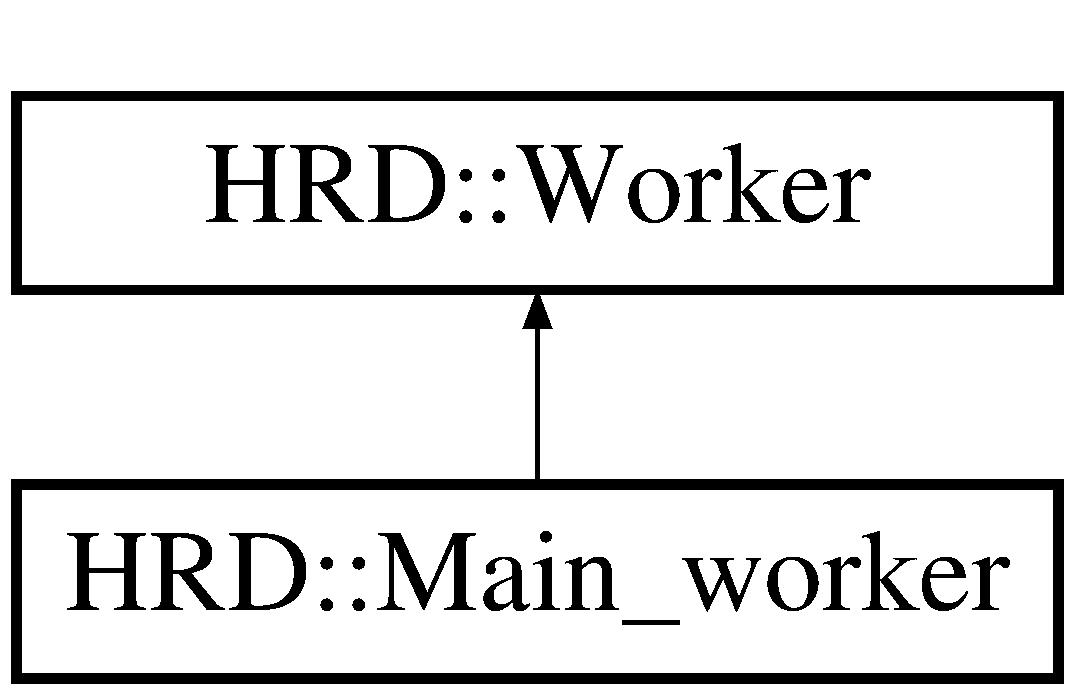
\includegraphics[height=2.000000cm]{class_h_r_d_1_1_main__worker}
\end{center}
\end{figure}
\subsection*{Public Member Functions}
\begin{DoxyCompactItemize}
\item 
\textbf{ Main\+\_\+worker} ()
\item 
\textbf{ Main\+\_\+worker} (char $\ast$\textbf{ name}, int \textbf{ year}, char $\ast$\textbf{ post}, char $\ast$\textbf{ educ}, int \textbf{ salary})
\item 
virtual \textbf{ Main\+\_\+worker} \& \textbf{ level\+\_\+up} ()
\item 
\textbf{ Unit} $\ast$ \textbf{ get\+\_\+\+Unit} () const
\item 
\textbf{ $\sim$\+Main\+\_\+worker} ()
\end{DoxyCompactItemize}
\subsection*{Public Attributes}
\begin{DoxyCompactItemize}
\item 
friend \textbf{ Us\+\_\+worker}
\end{DoxyCompactItemize}
\subsection*{Additional Inherited Members}


\subsection{Detailed Description}


Definition at line 29 of file \+\_\+\+Unit\+\_\+.\+h.



\subsection{Constructor \& Destructor Documentation}
\mbox{\label{class_h_r_d_1_1_main__worker_aa9100bfcf5c63371f8109c5bbaf81243}} 
\index{H\+R\+D\+::\+Main\+\_\+worker@{H\+R\+D\+::\+Main\+\_\+worker}!Main\+\_\+worker@{Main\+\_\+worker}}
\index{Main\+\_\+worker@{Main\+\_\+worker}!H\+R\+D\+::\+Main\+\_\+worker@{H\+R\+D\+::\+Main\+\_\+worker}}
\subsubsection{Main\+\_\+worker()\hspace{0.1cm}{\footnotesize\ttfamily [1/2]}}
{\footnotesize\ttfamily H\+R\+D\+::\+Main\+\_\+worker\+::\+Main\+\_\+worker (\begin{DoxyParamCaption}{ }\end{DoxyParamCaption})\hspace{0.3cm}{\ttfamily [inline]}}



Definition at line 34 of file \+\_\+\+Unit\+\_\+.\+h.

\mbox{\label{class_h_r_d_1_1_main__worker_a9a4c8c4a1a4cfe45db19555fe5dd3932}} 
\index{H\+R\+D\+::\+Main\+\_\+worker@{H\+R\+D\+::\+Main\+\_\+worker}!Main\+\_\+worker@{Main\+\_\+worker}}
\index{Main\+\_\+worker@{Main\+\_\+worker}!H\+R\+D\+::\+Main\+\_\+worker@{H\+R\+D\+::\+Main\+\_\+worker}}
\subsubsection{Main\+\_\+worker()\hspace{0.1cm}{\footnotesize\ttfamily [2/2]}}
{\footnotesize\ttfamily H\+R\+D\+::\+Main\+\_\+worker\+::\+Main\+\_\+worker (\begin{DoxyParamCaption}\item[{char $\ast$}]{name,  }\item[{int}]{year,  }\item[{char $\ast$}]{post,  }\item[{char $\ast$}]{educ,  }\item[{int}]{salary }\end{DoxyParamCaption})}



Definition at line 6 of file \+\_\+\+Main\+\_\+worker\+\_\+.\+cpp.

\mbox{\label{class_h_r_d_1_1_main__worker_abca8ac73ed5b366044c40398e21cf1f0}} 
\index{H\+R\+D\+::\+Main\+\_\+worker@{H\+R\+D\+::\+Main\+\_\+worker}!````~Main\+\_\+worker@{$\sim$\+Main\+\_\+worker}}
\index{````~Main\+\_\+worker@{$\sim$\+Main\+\_\+worker}!H\+R\+D\+::\+Main\+\_\+worker@{H\+R\+D\+::\+Main\+\_\+worker}}
\subsubsection{$\sim$\+Main\+\_\+worker()}
{\footnotesize\ttfamily H\+R\+D\+::\+Main\+\_\+worker\+::$\sim$\+Main\+\_\+worker (\begin{DoxyParamCaption}{ }\end{DoxyParamCaption})}



Definition at line 16 of file \+\_\+\+Main\+\_\+worker\+\_\+.\+cpp.



\subsection{Member Function Documentation}
\mbox{\label{class_h_r_d_1_1_main__worker_aa73038c5c049642e3c1d6b1f7bac4502}} 
\index{H\+R\+D\+::\+Main\+\_\+worker@{H\+R\+D\+::\+Main\+\_\+worker}!get\+\_\+\+Unit@{get\+\_\+\+Unit}}
\index{get\+\_\+\+Unit@{get\+\_\+\+Unit}!H\+R\+D\+::\+Main\+\_\+worker@{H\+R\+D\+::\+Main\+\_\+worker}}
\subsubsection{get\+\_\+\+Unit()}
{\footnotesize\ttfamily \textbf{ Unit}$\ast$ H\+R\+D\+::\+Main\+\_\+worker\+::get\+\_\+\+Unit (\begin{DoxyParamCaption}{ }\end{DoxyParamCaption}) const\hspace{0.3cm}{\ttfamily [inline]}}



Definition at line 38 of file \+\_\+\+Unit\+\_\+.\+h.

\mbox{\label{class_h_r_d_1_1_main__worker_a6d0d60e901294d4ff7ccbaee0254b0f3}} 
\index{H\+R\+D\+::\+Main\+\_\+worker@{H\+R\+D\+::\+Main\+\_\+worker}!level\+\_\+up@{level\+\_\+up}}
\index{level\+\_\+up@{level\+\_\+up}!H\+R\+D\+::\+Main\+\_\+worker@{H\+R\+D\+::\+Main\+\_\+worker}}
\subsubsection{level\+\_\+up()}
{\footnotesize\ttfamily virtual \textbf{ Main\+\_\+worker}\& H\+R\+D\+::\+Main\+\_\+worker\+::level\+\_\+up (\begin{DoxyParamCaption}{ }\end{DoxyParamCaption})\hspace{0.3cm}{\ttfamily [inline]}, {\ttfamily [virtual]}}



Implements \textbf{ H\+R\+D\+::\+Worker} \doxyref{}{p.}{class_h_r_d_1_1_worker_a67f5d9cc2dd74d1722419fca51d81770}.



Definition at line 36 of file \+\_\+\+Unit\+\_\+.\+h.



\subsection{Member Data Documentation}
\mbox{\label{class_h_r_d_1_1_main__worker_a1f1425e6932ebb5a777e7322db7d6453}} 
\index{H\+R\+D\+::\+Main\+\_\+worker@{H\+R\+D\+::\+Main\+\_\+worker}!Us\+\_\+worker@{Us\+\_\+worker}}
\index{Us\+\_\+worker@{Us\+\_\+worker}!H\+R\+D\+::\+Main\+\_\+worker@{H\+R\+D\+::\+Main\+\_\+worker}}
\subsubsection{Us\+\_\+worker}
{\footnotesize\ttfamily friend H\+R\+D\+::\+Main\+\_\+worker\+::\+Us\+\_\+worker}



Definition at line 37 of file \+\_\+\+Unit\+\_\+.\+h.



The documentation for this class was generated from the following files\+:\begin{DoxyCompactItemize}
\item 
C\+:/\+Users/\+Mixen/\+Desktop/Маслов Андрей/\+C++/\+I\+I\+I сем/\+Human\+\_\+\+Resources\+\_\+\+Department/\+Human\+\_\+\+Resources\+\_\+\+Department/\textbf{ \+\_\+\+Unit\+\_\+.\+h}\item 
C\+:/\+Users/\+Mixen/\+Desktop/Маслов Андрей/\+C++/\+I\+I\+I сем/\+Human\+\_\+\+Resources\+\_\+\+Department/\+Human\+\_\+\+Resources\+\_\+\+Department/\textbf{ \+\_\+\+Main\+\_\+worker\+\_\+.\+cpp}\end{DoxyCompactItemize}

\section{tab Struct Reference}
\label{structtab}\index{tab@{tab}}


{\ttfamily \#include $<$Structs.\+h$>$}

\subsection*{Public Attributes}
\begin{DoxyCompactItemize}
\item 
int \textbf{ n}
\item 
\textbf{ el\+\_\+tab} $\ast$ \textbf{ workers}
\end{DoxyCompactItemize}


\subsection{Detailed Description}


Definition at line 10 of file Structs.\+h.



\subsection{Member Data Documentation}
\mbox{\label{structtab_a277daf05539090402f78eb4d17f401a2}} 
\index{tab@{tab}!n@{n}}
\index{n@{n}!tab@{tab}}
\subsubsection{n}
{\footnotesize\ttfamily int tab\+::n}



Definition at line 12 of file Structs.\+h.

\mbox{\label{structtab_a6212e72593b78ec4ff8b660327602e79}} 
\index{tab@{tab}!workers@{workers}}
\index{workers@{workers}!tab@{tab}}
\subsubsection{workers}
{\footnotesize\ttfamily \textbf{ el\+\_\+tab}$\ast$ tab\+::workers}



Definition at line 13 of file Structs.\+h.



The documentation for this struct was generated from the following file\+:\begin{DoxyCompactItemize}
\item 
C\+:/\+Users/\+Mixen/\+Desktop/Маслов Андрей/\+C++/\+I\+I\+I сем/\+Human\+\_\+\+Resources\+\_\+\+Department/\+Human\+\_\+\+Resources\+\_\+\+Department/\textbf{ Structs.\+h}\end{DoxyCompactItemize}

\section{H\+RD\+:\+:Unit Class Reference}
\label{class_h_r_d_1_1_unit}\index{H\+R\+D\+::\+Unit@{H\+R\+D\+::\+Unit}}


{\ttfamily \#include $<$\+\_\+\+Unit\+\_\+.\+h$>$}

\subsection*{Public Member Functions}
\begin{DoxyCompactItemize}
\item 
\textbf{ Unit} \& \textbf{ add} (int, \textbf{ Worker} $\ast$)
\item 
auto \textbf{ find} (int chifr) const
\item 
auto \textbf{ find} (char $\ast$) const
\item 
\textbf{ Unit} \& \textbf{ del} (int)
\item 
char $\ast$ \textbf{ get\+Name} ()
\end{DoxyCompactItemize}
\subsection*{Friends}
\begin{DoxyCompactItemize}
\item 
std\+::ostream \& \textbf{ operator$<$$<$} (std\+::ostream \&, const \textbf{ Unit} \&)
\end{DoxyCompactItemize}


\subsection{Detailed Description}


Definition at line 11 of file \+\_\+\+Unit\+\_\+.\+h.



\subsection{Member Function Documentation}
\mbox{\label{class_h_r_d_1_1_unit_a2ebd571aada586d1a05507962ea0c7b0}} 
\index{H\+R\+D\+::\+Unit@{H\+R\+D\+::\+Unit}!add@{add}}
\index{add@{add}!H\+R\+D\+::\+Unit@{H\+R\+D\+::\+Unit}}
\subsubsection{add()}
{\footnotesize\ttfamily \textbf{ Unit} \& H\+R\+D\+::\+Unit\+::add (\begin{DoxyParamCaption}\item[{int}]{chifr,  }\item[{\textbf{ Worker} $\ast$}]{person }\end{DoxyParamCaption})}



Definition at line 6 of file \+\_\+\+Unit\+\_\+.\+cpp.

\mbox{\label{class_h_r_d_1_1_unit_a459dcefa63b6fe7086892e9831cc25fc}} 
\index{H\+R\+D\+::\+Unit@{H\+R\+D\+::\+Unit}!del@{del}}
\index{del@{del}!H\+R\+D\+::\+Unit@{H\+R\+D\+::\+Unit}}
\subsubsection{del()}
{\footnotesize\ttfamily \textbf{ Unit} \& H\+R\+D\+::\+Unit\+::del (\begin{DoxyParamCaption}\item[{int}]{chifr }\end{DoxyParamCaption})}



Definition at line 21 of file \+\_\+\+Unit\+\_\+.\+cpp.

\mbox{\label{class_h_r_d_1_1_unit_aa9e4bc8f93ec30cdee2266edaab22024}} 
\index{H\+R\+D\+::\+Unit@{H\+R\+D\+::\+Unit}!find@{find}}
\index{find@{find}!H\+R\+D\+::\+Unit@{H\+R\+D\+::\+Unit}}
\subsubsection{find()\hspace{0.1cm}{\footnotesize\ttfamily [1/2]}}
{\footnotesize\ttfamily auto H\+R\+D\+::\+Unit\+::find (\begin{DoxyParamCaption}\item[{int}]{chifr }\end{DoxyParamCaption}) const\hspace{0.3cm}{\ttfamily [inline]}}



Definition at line 18 of file \+\_\+\+Unit\+\_\+.\+h.

\mbox{\label{class_h_r_d_1_1_unit_a30bd9a6e7dcc61bb60a41080b61ca132}} 
\index{H\+R\+D\+::\+Unit@{H\+R\+D\+::\+Unit}!find@{find}}
\index{find@{find}!H\+R\+D\+::\+Unit@{H\+R\+D\+::\+Unit}}
\subsubsection{find()\hspace{0.1cm}{\footnotesize\ttfamily [2/2]}}
{\footnotesize\ttfamily auto H\+R\+D\+::\+Unit\+::find (\begin{DoxyParamCaption}\item[{char $\ast$}]{unit }\end{DoxyParamCaption}) const}



Definition at line 12 of file \+\_\+\+Unit\+\_\+.\+cpp.

\mbox{\label{class_h_r_d_1_1_unit_ae182e56ce7319b2ff4824c5ba7a7f945}} 
\index{H\+R\+D\+::\+Unit@{H\+R\+D\+::\+Unit}!get\+Name@{get\+Name}}
\index{get\+Name@{get\+Name}!H\+R\+D\+::\+Unit@{H\+R\+D\+::\+Unit}}
\subsubsection{get\+Name()}
{\footnotesize\ttfamily char$\ast$ H\+R\+D\+::\+Unit\+::get\+Name (\begin{DoxyParamCaption}{ }\end{DoxyParamCaption})\hspace{0.3cm}{\ttfamily [inline]}}



Definition at line 21 of file \+\_\+\+Unit\+\_\+.\+h.



\subsection{Friends And Related Function Documentation}
\mbox{\label{class_h_r_d_1_1_unit_ac0bce1523e9a2843a631a23662ac239b}} 
\index{H\+R\+D\+::\+Unit@{H\+R\+D\+::\+Unit}!operator$<$$<$@{operator$<$$<$}}
\index{operator$<$$<$@{operator$<$$<$}!H\+R\+D\+::\+Unit@{H\+R\+D\+::\+Unit}}
\subsubsection{operator$<$$<$}
{\footnotesize\ttfamily std\+::ostream\& operator$<$$<$ (\begin{DoxyParamCaption}\item[{std\+::ostream \&}]{s,  }\item[{const \textbf{ Unit} \&}]{st }\end{DoxyParamCaption})\hspace{0.3cm}{\ttfamily [friend]}}



Definition at line 27 of file \+\_\+\+Unit\+\_\+.\+cpp.



The documentation for this class was generated from the following files\+:\begin{DoxyCompactItemize}
\item 
\textbf{ \+\_\+\+Unit\+\_\+.\+h}\item 
\textbf{ \+\_\+\+Unit\+\_\+.\+cpp}\end{DoxyCompactItemize}

\section{H\+RD\+:\+:Us\+\_\+worker Class Reference}
\label{class_h_r_d_1_1_us__worker}\index{H\+R\+D\+::\+Us\+\_\+worker@{H\+R\+D\+::\+Us\+\_\+worker}}


{\ttfamily \#include $<$\+\_\+\+Unit\+\_\+.\+h$>$}

Inheritance diagram for H\+RD\+:\+:Us\+\_\+worker\+:\begin{figure}[H]
\begin{center}
\leavevmode
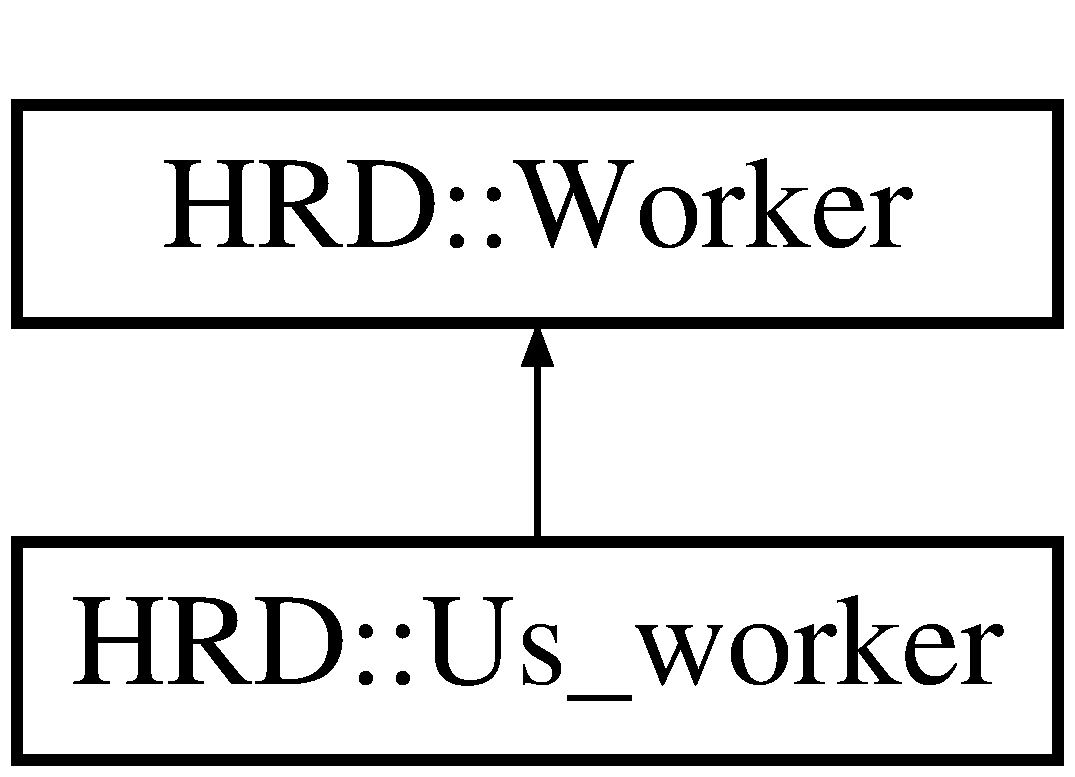
\includegraphics[height=2.000000cm]{class_h_r_d_1_1_us__worker}
\end{center}
\end{figure}
\subsection*{Public Member Functions}
\begin{DoxyCompactItemize}
\item 
\textbf{ Us\+\_\+worker} ()
\item 
\textbf{ Us\+\_\+worker} (char $\ast$\textbf{ name}, int \textbf{ year}, char $\ast$\textbf{ post}, char $\ast$\textbf{ educ}, int \textbf{ salary})
\item 
\textbf{ Main\+\_\+worker} \& \textbf{ level\+\_\+up} (\textbf{ Unit} $\ast$)
\item 
\textbf{ $\sim$\+Us\+\_\+worker} ()
\end{DoxyCompactItemize}
\subsection*{Additional Inherited Members}


\subsection{Detailed Description}


Definition at line 42 of file \+\_\+\+Unit\+\_\+.\+h.



\subsection{Constructor \& Destructor Documentation}
\mbox{\label{class_h_r_d_1_1_us__worker_a7e0c8b11ec80568a7905abd13b4681f5}} 
\index{H\+R\+D\+::\+Us\+\_\+worker@{H\+R\+D\+::\+Us\+\_\+worker}!Us\+\_\+worker@{Us\+\_\+worker}}
\index{Us\+\_\+worker@{Us\+\_\+worker}!H\+R\+D\+::\+Us\+\_\+worker@{H\+R\+D\+::\+Us\+\_\+worker}}
\subsubsection{Us\+\_\+worker()\hspace{0.1cm}{\footnotesize\ttfamily [1/2]}}
{\footnotesize\ttfamily H\+R\+D\+::\+Us\+\_\+worker\+::\+Us\+\_\+worker (\begin{DoxyParamCaption}{ }\end{DoxyParamCaption})\hspace{0.3cm}{\ttfamily [inline]}}



Definition at line 45 of file \+\_\+\+Unit\+\_\+.\+h.

\mbox{\label{class_h_r_d_1_1_us__worker_ac0a6cff72a4b5f7f4f26e5a336f25c91}} 
\index{H\+R\+D\+::\+Us\+\_\+worker@{H\+R\+D\+::\+Us\+\_\+worker}!Us\+\_\+worker@{Us\+\_\+worker}}
\index{Us\+\_\+worker@{Us\+\_\+worker}!H\+R\+D\+::\+Us\+\_\+worker@{H\+R\+D\+::\+Us\+\_\+worker}}
\subsubsection{Us\+\_\+worker()\hspace{0.1cm}{\footnotesize\ttfamily [2/2]}}
{\footnotesize\ttfamily H\+R\+D\+::\+Us\+\_\+worker\+::\+Us\+\_\+worker (\begin{DoxyParamCaption}\item[{char $\ast$}]{name,  }\item[{int}]{year,  }\item[{char $\ast$}]{post,  }\item[{char $\ast$}]{educ,  }\item[{int}]{salary }\end{DoxyParamCaption})}



Definition at line 6 of file \+\_\+\+Us\+\_\+worker\+\_\+.\+cpp.

\mbox{\label{class_h_r_d_1_1_us__worker_ae14459b2b134dc0561abca6132027ccd}} 
\index{H\+R\+D\+::\+Us\+\_\+worker@{H\+R\+D\+::\+Us\+\_\+worker}!````~Us\+\_\+worker@{$\sim$\+Us\+\_\+worker}}
\index{````~Us\+\_\+worker@{$\sim$\+Us\+\_\+worker}!H\+R\+D\+::\+Us\+\_\+worker@{H\+R\+D\+::\+Us\+\_\+worker}}
\subsubsection{$\sim$\+Us\+\_\+worker()}
{\footnotesize\ttfamily H\+R\+D\+::\+Us\+\_\+worker\+::$\sim$\+Us\+\_\+worker (\begin{DoxyParamCaption}{ }\end{DoxyParamCaption})}



Definition at line 29 of file \+\_\+\+Us\+\_\+worker\+\_\+.\+cpp.



\subsection{Member Function Documentation}
\mbox{\label{class_h_r_d_1_1_us__worker_ab5059f9f2a77131ca271081d36e77080}} 
\index{H\+R\+D\+::\+Us\+\_\+worker@{H\+R\+D\+::\+Us\+\_\+worker}!level\+\_\+up@{level\+\_\+up}}
\index{level\+\_\+up@{level\+\_\+up}!H\+R\+D\+::\+Us\+\_\+worker@{H\+R\+D\+::\+Us\+\_\+worker}}
\subsubsection{level\+\_\+up()}
{\footnotesize\ttfamily \textbf{ Main\+\_\+worker} \& H\+R\+D\+::\+Us\+\_\+worker\+::level\+\_\+up (\begin{DoxyParamCaption}\item[{\textbf{ Unit} $\ast$}]{up }\end{DoxyParamCaption})}



Definition at line 16 of file \+\_\+\+Us\+\_\+worker\+\_\+.\+cpp.



The documentation for this class was generated from the following files\+:\begin{DoxyCompactItemize}
\item 
C\+:/\+Users/\+Mixen/\+Desktop/Маслов Андрей/\+C++/\+I\+I\+I сем/\+Human\+\_\+\+Resources\+\_\+\+Department/\+Human\+\_\+\+Resources\+\_\+\+Department/\textbf{ \+\_\+\+Unit\+\_\+.\+h}\item 
C\+:/\+Users/\+Mixen/\+Desktop/Маслов Андрей/\+C++/\+I\+I\+I сем/\+Human\+\_\+\+Resources\+\_\+\+Department/\+Human\+\_\+\+Resources\+\_\+\+Department/\textbf{ \+\_\+\+Us\+\_\+worker\+\_\+.\+cpp}\end{DoxyCompactItemize}

\section{H\+RD\+:\+:Worker Class Reference}
\label{class_h_r_d_1_1_worker}\index{H\+R\+D\+::\+Worker@{H\+R\+D\+::\+Worker}}


{\ttfamily \#include $<$\+\_\+\+Worker\+\_\+.\+h$>$}

Inheritance diagram for H\+RD\+:\+:Worker\+:\begin{figure}[H]
\begin{center}
\leavevmode
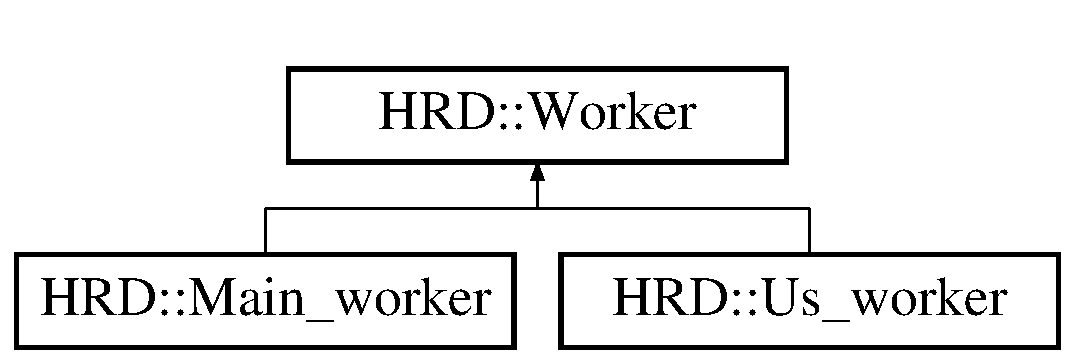
\includegraphics[height=2.000000cm]{class_h_r_d_1_1_worker}
\end{center}
\end{figure}
\subsection*{Public Member Functions}
\begin{DoxyCompactItemize}
\item 
virtual \textbf{ Unit} $\ast$ \textbf{ get\+\_\+\+Unit} ()=0
\item 
int \textbf{ info} ()
\item 
int \textbf{ get\+\_\+type} ()
\item 
char $\ast$ \textbf{ get\+\_\+post} ()
\item 
\textbf{ Worker} \& \textbf{ ch\+\_\+\+Post} (char $\ast$)
\item 
int \textbf{ get\+Salary} ()
\item 
\textbf{ Worker} \& \textbf{ ch\+\_\+\+Salary} (int)
\item 
virtual \textbf{ Worker} \& \textbf{ level\+\_\+up} ()=0
\end{DoxyCompactItemize}
\subsection*{Protected Attributes}
\begin{DoxyCompactItemize}
\item 
char $\ast$ \textbf{ name}
\item 
int \textbf{ year}
\item 
char $\ast$ \textbf{ post}
\item 
char $\ast$ \textbf{ educ}
\item 
int \textbf{ salary}
\item 
int \textbf{ type}
\end{DoxyCompactItemize}


\subsection{Detailed Description}


Definition at line 8 of file \+\_\+\+Worker\+\_\+.\+h.



\subsection{Member Function Documentation}
\mbox{\label{class_h_r_d_1_1_worker_a9234599c0ef3b17151b7e8a813e28581}} 
\index{H\+R\+D\+::\+Worker@{H\+R\+D\+::\+Worker}!ch\+\_\+\+Post@{ch\+\_\+\+Post}}
\index{ch\+\_\+\+Post@{ch\+\_\+\+Post}!H\+R\+D\+::\+Worker@{H\+R\+D\+::\+Worker}}
\subsubsection{ch\+\_\+\+Post()}
{\footnotesize\ttfamily \textbf{ Worker} \& H\+R\+D\+::\+Worker\+::ch\+\_\+\+Post (\begin{DoxyParamCaption}\item[{char $\ast$}]{new\+\_\+post }\end{DoxyParamCaption})}



Definition at line 30 of file \+\_\+\+Worker\+\_\+.\+cpp.

\mbox{\label{class_h_r_d_1_1_worker_a3d0ea5e210bd344170866c32ca5013da}} 
\index{H\+R\+D\+::\+Worker@{H\+R\+D\+::\+Worker}!ch\+\_\+\+Salary@{ch\+\_\+\+Salary}}
\index{ch\+\_\+\+Salary@{ch\+\_\+\+Salary}!H\+R\+D\+::\+Worker@{H\+R\+D\+::\+Worker}}
\subsubsection{ch\+\_\+\+Salary()}
{\footnotesize\ttfamily \textbf{ Worker} \& H\+R\+D\+::\+Worker\+::ch\+\_\+\+Salary (\begin{DoxyParamCaption}\item[{int}]{new\+\_\+salary }\end{DoxyParamCaption})}



Definition at line 37 of file \+\_\+\+Worker\+\_\+.\+cpp.

\mbox{\label{class_h_r_d_1_1_worker_a9e358b8861e16955d6fb11600a144782}} 
\index{H\+R\+D\+::\+Worker@{H\+R\+D\+::\+Worker}!get\+\_\+post@{get\+\_\+post}}
\index{get\+\_\+post@{get\+\_\+post}!H\+R\+D\+::\+Worker@{H\+R\+D\+::\+Worker}}
\subsubsection{get\+\_\+post()}
{\footnotesize\ttfamily char$\ast$ H\+R\+D\+::\+Worker\+::get\+\_\+post (\begin{DoxyParamCaption}{ }\end{DoxyParamCaption})\hspace{0.3cm}{\ttfamily [inline]}}



Definition at line 21 of file \+\_\+\+Worker\+\_\+.\+h.

\mbox{\label{class_h_r_d_1_1_worker_a36d91b12e9921bd9b0c3a00bb1dde041}} 
\index{H\+R\+D\+::\+Worker@{H\+R\+D\+::\+Worker}!get\+\_\+type@{get\+\_\+type}}
\index{get\+\_\+type@{get\+\_\+type}!H\+R\+D\+::\+Worker@{H\+R\+D\+::\+Worker}}
\subsubsection{get\+\_\+type()}
{\footnotesize\ttfamily int H\+R\+D\+::\+Worker\+::get\+\_\+type (\begin{DoxyParamCaption}{ }\end{DoxyParamCaption})}



Definition at line 16 of file \+\_\+\+Worker\+\_\+.\+cpp.

\mbox{\label{class_h_r_d_1_1_worker_a9938987a0bc823d8492767df29631821}} 
\index{H\+R\+D\+::\+Worker@{H\+R\+D\+::\+Worker}!get\+\_\+\+Unit@{get\+\_\+\+Unit}}
\index{get\+\_\+\+Unit@{get\+\_\+\+Unit}!H\+R\+D\+::\+Worker@{H\+R\+D\+::\+Worker}}
\subsubsection{get\+\_\+\+Unit()}
{\footnotesize\ttfamily virtual \textbf{ Unit}$\ast$ H\+R\+D\+::\+Worker\+::get\+\_\+\+Unit (\begin{DoxyParamCaption}{ }\end{DoxyParamCaption})\hspace{0.3cm}{\ttfamily [pure virtual]}}

\mbox{\label{class_h_r_d_1_1_worker_a517416984f3a6b7632fa484dfc8f950f}} 
\index{H\+R\+D\+::\+Worker@{H\+R\+D\+::\+Worker}!get\+Salary@{get\+Salary}}
\index{get\+Salary@{get\+Salary}!H\+R\+D\+::\+Worker@{H\+R\+D\+::\+Worker}}
\subsubsection{get\+Salary()}
{\footnotesize\ttfamily int H\+R\+D\+::\+Worker\+::get\+Salary (\begin{DoxyParamCaption}{ }\end{DoxyParamCaption})\hspace{0.3cm}{\ttfamily [inline]}}



Definition at line 23 of file \+\_\+\+Worker\+\_\+.\+h.

\mbox{\label{class_h_r_d_1_1_worker_a0a1c1ddb9f1b89ad00e22f09b0004e34}} 
\index{H\+R\+D\+::\+Worker@{H\+R\+D\+::\+Worker}!info@{info}}
\index{info@{info}!H\+R\+D\+::\+Worker@{H\+R\+D\+::\+Worker}}
\subsubsection{info()}
{\footnotesize\ttfamily int H\+R\+D\+::\+Worker\+::info (\begin{DoxyParamCaption}{ }\end{DoxyParamCaption})}



Definition at line 6 of file \+\_\+\+Worker\+\_\+.\+cpp.

\mbox{\label{class_h_r_d_1_1_worker_a67f5d9cc2dd74d1722419fca51d81770}} 
\index{H\+R\+D\+::\+Worker@{H\+R\+D\+::\+Worker}!level\+\_\+up@{level\+\_\+up}}
\index{level\+\_\+up@{level\+\_\+up}!H\+R\+D\+::\+Worker@{H\+R\+D\+::\+Worker}}
\subsubsection{level\+\_\+up()}
{\footnotesize\ttfamily virtual \textbf{ Worker}\& H\+R\+D\+::\+Worker\+::level\+\_\+up (\begin{DoxyParamCaption}{ }\end{DoxyParamCaption})\hspace{0.3cm}{\ttfamily [pure virtual]}}



Implemented in \textbf{ H\+R\+D\+::\+Main\+\_\+worker} \doxyref{}{p.}{class_h_r_d_1_1_main__worker_a6d0d60e901294d4ff7ccbaee0254b0f3}.



\subsection{Member Data Documentation}
\mbox{\label{class_h_r_d_1_1_worker_afdea20210e05fd323929277bbbd59b55}} 
\index{H\+R\+D\+::\+Worker@{H\+R\+D\+::\+Worker}!educ@{educ}}
\index{educ@{educ}!H\+R\+D\+::\+Worker@{H\+R\+D\+::\+Worker}}
\subsubsection{educ}
{\footnotesize\ttfamily char$\ast$ H\+R\+D\+::\+Worker\+::educ\hspace{0.3cm}{\ttfamily [protected]}}



Definition at line 14 of file \+\_\+\+Worker\+\_\+.\+h.

\mbox{\label{class_h_r_d_1_1_worker_af94f6c3ee6d8a33d6383fcc71ec90c51}} 
\index{H\+R\+D\+::\+Worker@{H\+R\+D\+::\+Worker}!name@{name}}
\index{name@{name}!H\+R\+D\+::\+Worker@{H\+R\+D\+::\+Worker}}
\subsubsection{name}
{\footnotesize\ttfamily char$\ast$ H\+R\+D\+::\+Worker\+::name\hspace{0.3cm}{\ttfamily [protected]}}



Definition at line 11 of file \+\_\+\+Worker\+\_\+.\+h.

\mbox{\label{class_h_r_d_1_1_worker_a3d4dbc1be974cd3862be4b300a29d16f}} 
\index{H\+R\+D\+::\+Worker@{H\+R\+D\+::\+Worker}!post@{post}}
\index{post@{post}!H\+R\+D\+::\+Worker@{H\+R\+D\+::\+Worker}}
\subsubsection{post}
{\footnotesize\ttfamily char$\ast$ H\+R\+D\+::\+Worker\+::post\hspace{0.3cm}{\ttfamily [protected]}}



Definition at line 13 of file \+\_\+\+Worker\+\_\+.\+h.

\mbox{\label{class_h_r_d_1_1_worker_a82ca5a4ad2e0347f4fa663519f14550f}} 
\index{H\+R\+D\+::\+Worker@{H\+R\+D\+::\+Worker}!salary@{salary}}
\index{salary@{salary}!H\+R\+D\+::\+Worker@{H\+R\+D\+::\+Worker}}
\subsubsection{salary}
{\footnotesize\ttfamily int H\+R\+D\+::\+Worker\+::salary\hspace{0.3cm}{\ttfamily [protected]}}



Definition at line 15 of file \+\_\+\+Worker\+\_\+.\+h.

\mbox{\label{class_h_r_d_1_1_worker_acfdaa671f5b87e440310da74d89ffe85}} 
\index{H\+R\+D\+::\+Worker@{H\+R\+D\+::\+Worker}!type@{type}}
\index{type@{type}!H\+R\+D\+::\+Worker@{H\+R\+D\+::\+Worker}}
\subsubsection{type}
{\footnotesize\ttfamily int H\+R\+D\+::\+Worker\+::type\hspace{0.3cm}{\ttfamily [protected]}}



Definition at line 16 of file \+\_\+\+Worker\+\_\+.\+h.

\mbox{\label{class_h_r_d_1_1_worker_a2db533aa6e323c5f55dd3d9c9c786d13}} 
\index{H\+R\+D\+::\+Worker@{H\+R\+D\+::\+Worker}!year@{year}}
\index{year@{year}!H\+R\+D\+::\+Worker@{H\+R\+D\+::\+Worker}}
\subsubsection{year}
{\footnotesize\ttfamily int H\+R\+D\+::\+Worker\+::year\hspace{0.3cm}{\ttfamily [protected]}}



Definition at line 12 of file \+\_\+\+Worker\+\_\+.\+h.



The documentation for this class was generated from the following files\+:\begin{DoxyCompactItemize}
\item 
C\+:/\+Users/\+Mixen/\+Desktop/Маслов Андрей/\+C++/\+I\+I\+I сем/\+Human\+\_\+\+Resources\+\_\+\+Department/\+Human\+\_\+\+Resources\+\_\+\+Department/\textbf{ \+\_\+\+Worker\+\_\+.\+h}\item 
C\+:/\+Users/\+Mixen/\+Desktop/Маслов Андрей/\+C++/\+I\+I\+I сем/\+Human\+\_\+\+Resources\+\_\+\+Department/\+Human\+\_\+\+Resources\+\_\+\+Department/\textbf{ \+\_\+\+Worker\+\_\+.\+cpp}\end{DoxyCompactItemize}

\chapter{File Documentation}
\section{C\+:/\+Users/\+Mixen/\+Desktop/Маслов Андрей/\+C++/\+I\+II сем/\+Human\+\_\+\+Resources\+\_\+\+Department/\+Human\+\_\+\+Resources\+\_\+\+Department/\+\_\+\+Main\+\_\+worker\+\_\+.cpp File Reference}
\label{___main__worker___8cpp}\index{C\+:/\+Users/\+Mixen/\+Desktop/Маслов Андрей/\+C++/\+I\+I\+I сем/\+Human\+\_\+\+Resources\+\_\+\+Department/\+Human\+\_\+\+Resources\+\_\+\+Department/\+\_\+\+Main\+\_\+worker\+\_\+.\+cpp@{C\+:/\+Users/\+Mixen/\+Desktop/Маслов Андрей/\+C++/\+I\+I\+I сем/\+Human\+\_\+\+Resources\+\_\+\+Department/\+Human\+\_\+\+Resources\+\_\+\+Department/\+\_\+\+Main\+\_\+worker\+\_\+.\+cpp}}
{\ttfamily \#include \char`\"{}\+\_\+\+Unit\+\_\+.\+h\char`\"{}}\newline
\subsection*{Namespaces}
\begin{DoxyCompactItemize}
\item 
 \textbf{ H\+RD}
\end{DoxyCompactItemize}

\section{\+\_\+\+Unit\+\_\+.\+cpp File Reference}
\label{___unit___8cpp}\index{\+\_\+\+Unit\+\_\+.\+cpp@{\+\_\+\+Unit\+\_\+.\+cpp}}
{\ttfamily \#include \char`\"{}\+\_\+\+Unit\+\_\+.\+h\char`\"{}}\newline
\subsection*{Namespaces}
\begin{DoxyCompactItemize}
\item 
 \textbf{ H\+RD}
\end{DoxyCompactItemize}
\subsection*{Functions}
\begin{DoxyCompactItemize}
\item 
std\+::ostream \& \textbf{ H\+R\+D\+::operator$<$$<$} (std\+::ostream \&s, const \textbf{ Unit} \&st)
\end{DoxyCompactItemize}

\section{\+\_\+\+Unit\+\_\+.\+h File Reference}
\label{___unit___8h}\index{\+\_\+\+Unit\+\_\+.\+h@{\+\_\+\+Unit\+\_\+.\+h}}
{\ttfamily \#include $<$map$>$}\newline
{\ttfamily \#include \char`\"{}\+\_\+\+Worker\+\_\+.\+h\char`\"{}}\newline
{\ttfamily \#include $<$iostream$>$}\newline
\subsection*{Classes}
\begin{DoxyCompactItemize}
\item 
class \textbf{ H\+R\+D\+::\+Unit}
\item 
class \textbf{ H\+R\+D\+::\+Main\+\_\+worker}
\item 
class \textbf{ H\+R\+D\+::\+Us\+\_\+worker}
\end{DoxyCompactItemize}
\subsection*{Namespaces}
\begin{DoxyCompactItemize}
\item 
 \textbf{ H\+RD}
\end{DoxyCompactItemize}

\section{\+\_\+\+Us\+\_\+worker\+\_\+.\+cpp File Reference}
\label{___us__worker___8cpp}\index{\+\_\+\+Us\+\_\+worker\+\_\+.\+cpp@{\+\_\+\+Us\+\_\+worker\+\_\+.\+cpp}}
{\ttfamily \#include \char`\"{}\+\_\+\+Unit\+\_\+.\+h\char`\"{}}\newline
\subsection*{Namespaces}
\begin{DoxyCompactItemize}
\item 
 \textbf{ H\+RD}
\end{DoxyCompactItemize}

\section{\+\_\+\+Worker\+\_\+.\+cpp File Reference}
\label{___worker___8cpp}\index{\+\_\+\+Worker\+\_\+.\+cpp@{\+\_\+\+Worker\+\_\+.\+cpp}}
{\ttfamily \#include \char`\"{}\+\_\+\+Worker\+\_\+.\+h\char`\"{}}\newline
\subsection*{Namespaces}
\begin{DoxyCompactItemize}
\item 
 \textbf{ H\+RD}
\end{DoxyCompactItemize}

\section{C\+:/\+Users/\+Mixen/\+Desktop/Маслов Андрей/\+C++/\+I\+II сем/\+Human\+\_\+\+Resources\+\_\+\+Department/\+Human\+\_\+\+Resources\+\_\+\+Department/\+\_\+\+Worker\+\_\+.h File Reference}
\label{___worker___8h}\index{C\+:/\+Users/\+Mixen/\+Desktop/Маслов Андрей/\+C++/\+I\+I\+I сем/\+Human\+\_\+\+Resources\+\_\+\+Department/\+Human\+\_\+\+Resources\+\_\+\+Department/\+\_\+\+Worker\+\_\+.\+h@{C\+:/\+Users/\+Mixen/\+Desktop/Маслов Андрей/\+C++/\+I\+I\+I сем/\+Human\+\_\+\+Resources\+\_\+\+Department/\+Human\+\_\+\+Resources\+\_\+\+Department/\+\_\+\+Worker\+\_\+.\+h}}
{\ttfamily \#include $<$iostream$>$}\newline
\subsection*{Classes}
\begin{DoxyCompactItemize}
\item 
class \textbf{ H\+R\+D\+::\+Worker}
\end{DoxyCompactItemize}
\subsection*{Namespaces}
\begin{DoxyCompactItemize}
\item 
 \textbf{ H\+RD}
\end{DoxyCompactItemize}

\section{Human\+\_\+\+Resources\+\_\+\+Department.\+cpp File Reference}
\label{_human___resources___department_8cpp}\index{Human\+\_\+\+Resources\+\_\+\+Department.\+cpp@{Human\+\_\+\+Resources\+\_\+\+Department.\+cpp}}
{\ttfamily \#include $<$iostream$>$}\newline
\subsection*{Functions}
\begin{DoxyCompactItemize}
\item 
int \textbf{ main} ()
\end{DoxyCompactItemize}


\subsection{Function Documentation}
\mbox{\label{_human___resources___department_8cpp_ae66f6b31b5ad750f1fe042a706a4e3d4}} 
\index{Human\+\_\+\+Resources\+\_\+\+Department.\+cpp@{Human\+\_\+\+Resources\+\_\+\+Department.\+cpp}!main@{main}}
\index{main@{main}!Human\+\_\+\+Resources\+\_\+\+Department.\+cpp@{Human\+\_\+\+Resources\+\_\+\+Department.\+cpp}}
\subsubsection{main()}
{\footnotesize\ttfamily int main (\begin{DoxyParamCaption}{ }\end{DoxyParamCaption})}



Definition at line 7 of file Human\+\_\+\+Resources\+\_\+\+Department.\+cpp.


\section{Structs.\+h File Reference}
\label{_structs_8h}\index{Structs.\+h@{Structs.\+h}}
{\ttfamily \#include \char`\"{}\+\_\+\+Worker\+\_\+.\+h\char`\"{}}\newline
\subsection*{Classes}
\begin{DoxyCompactItemize}
\item 
struct \textbf{ el\+\_\+tab}
\item 
struct \textbf{ tab}
\end{DoxyCompactItemize}

%--- End generated contents ---

% Index
\backmatter
\newpage
\phantomsection
\clearemptydoublepage
\addcontentsline{toc}{chapter}{Index}
\printindex

\end{document}
